\documentclass{standalone}
    \usepackage{tikz}
    \usepackage{amsfonts}
    \begin{document}
    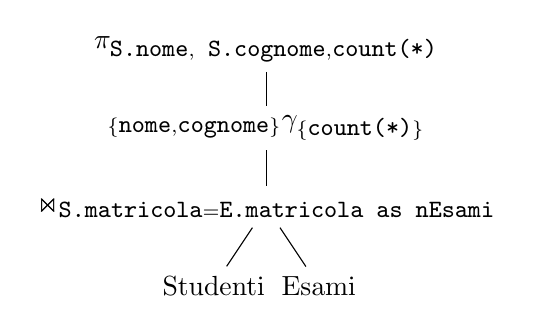
\begin{tikzpicture}\node (node) at (0, -1){$\pi_{\small\texttt{S.nome},\small\texttt{ S.cognome},\small\texttt{count(*)}}$};
\node (node0) at (0, -2){$_{\{\small\texttt{nome},\small\texttt{cognome}\}}\gamma_{\{\small\texttt{count(*)}\}}$};
\node (node00) at (0, -3){$\Join_{ \small\texttt{S.matricola}=\texttt{E.matricola as nEsami}}$};
\node (node000) at (-0.6666666666666666, -4){Studenti};
\node (node001) at (0.6666666666666666, -4){Esami};
\draw(node) -- (node0);
\draw(node0) -- (node00);
\draw(node00) -- (node000);
\draw(node00) -- (node001);
\end{tikzpicture}

\end{document}
